
\documentclass[a4paper,11pt,norsk]{article}
\usepackage[utf8]{inputenc}
%\usepackage[utf8]{inputenc}
\usepackage{a4wide}
\usepackage{lmodern}
\usepackage[T1]{fontenc}
\usepackage{babel}
\setlength{\parindent}{0pt} 
\setlength{\parskip}{2ex}
\usepackage{fixltx2e}
\usepackage{amsmath}
\usepackage[pdftex, pdfborderstyle={/S/U/W 0}]{hyperref}
\usepackage{graphicx}
\usepackage[font=small,labelfont=bf]{caption}
\usepackage{}
\usepackage{tabularx}
\usepackage{multirow}
\usepackage[american]{circuitikz}
\usetikzlibrary{arrows,shapes,positioning,calc}
\usetikzlibrary{decorations.markings}

\begin{document}

%Headingdel:---------------------------------------------
\begin{minipage}[c]{0.15\textwidth}

\includegraphics[width=2.0cm]{elsys_pos_staaende_ntnu}  
\end{minipage}
\begin{minipage}[c]{0.85\textwidth}

\renewcommand{\arraystretch}{1.7}
\large 
\begin{tabularx}{\textwidth}{|X|X|}
\hline
\multicolumn{2}{|l|}{} \\
\multicolumn{2}{|l|}{\huge \textbf{Rapport Arbeider 2}} \\
\multicolumn{2}{|l|}{}  \\
\hline
\multicolumn{2}{|l|}{Tittel: 
%Skriv inn tittel her:------------------------------------------
Frekvenssignatur for radiofyr (analogt design)
} \\
\hline
\multicolumn{2}{|l|}{Forfattere: 
%Skriv inn forfattere her:--------------------------------------
Sindre Danielsen
} \\
\hline
%Skriv inn versjon og dato her her:-----------------------------
Versjon: 1.0 & Dato: 05.12.21
\\
\hline 
\end{tabularx}
\end{minipage}
\normalsize

%Automatisk generert innholdsfortegnelse:------------------

\setlength{\parskip}{0ex}
\renewcommand{\baselinestretch}{0.1}\normalsize
\tableofcontents
\renewcommand{\baselinestretch}{1.00}\normalsize
\setlength{\parskip}{2ex}
\rule{\textwidth}{1pt}

%Selve rapporten:------------------------------------------
\newpage
\section{Problembeskrivelse}
\label{sec: problembeskrivelse}
Fly og skipsfartøy har mange metoder for å navigere og forstå sin posisjon. Eksempler på det er via satelitt eller kompass. En annen metode er å bruke \textit{radiofyr}. Det er en radiosender som sender ut et kjenningssignal (signatur) $x(t)$, slik at fartøyene kan fange opp signalene og tolke hvor de befinner seg. Et slikt kjenningssignal kan utvikles ved bruk av amplitudemodulasjon (AM) eller frekvensmodulasjon (FM). Metoden som skal utforskes her, er gjennom et signal som bytter mellom to betydelig ulike frekvenser $f_1$ og $f_2$ på et tidsintervall $T$.
En visuell representasjon er vist ved figur~\ref{fig: visuell FM}.
\\
\begin{figure}[!htbp]
    \centering
    \includegraphics[width=1.0\textwidth]{img/FM signal.png}
    \caption{Frekvensskifter: Signal som bytter mellom to frekvenser på et tidsintervall.}
    \label{fig: visuell FM}
\end{figure} \\
Mønsteret fra figuren repeteres kontinuerlig og kan representeres matematisk ved
\begin{equation*}
    x(t) =   
    \begin{cases}
    \cos{(2\pi f_1 t + \phi_1)} \quad \textrm{for} & t\in[kT, (k+1)T] \textrm{ for } k \textrm{ partall.}\\
    \cos{(2\pi f_2 t + \phi_2)} \quad \textrm{for} & t\in[kT, (k+1)T] \textrm{ for } k \textrm{ oddetall.}
    \end{cases}
\end{equation*}
Her tar vi hensyn til at de to frekvensene er på en tilnærmet sinusform. Faseforskyvningene $\phi_1$ og $\phi_2$ kan gjøre signalet kontinuerlig, men det blir ikke tatt med i betrakningen for utviklingen av systemet. \\
\\
Et problem som kan oppstå er at radiosignaler kan forstyrre hverandre. Det kan løses ved å ha kontroll over båndbredden $B$ på kjenningssignalet. For utviklingen av signalet her, så brukes 10dB-båndbredden (der signalets effektspekter $P_x(f)\in[0, -10]$dB). Se figur~\ref{fig: effektspekter}. \newpage
\begin{figure}[!hbtp]
    \centering
    \includegraphics[width=1.0\textwidth]{img/Effektspekter.png}
    \caption{Effektspekter på 10dB-båndbredde.}
    \label{fig: effektspekter}
\end{figure} \\

\newpage
\section{Prinsipiell løsning}
\label{sec: prinsipiell losning}
For utvikling av et system gitt i seksjon~\ref{sec: problembeskrivelse}, så kreves flere delsystemer. Det kan gjøres på forskjellige metoder, men her velges det å bruke en ulineær oscillator og transistorer. Valget fremkommer av at det er kun to frekvenser som skal brukes, så det er da ganske enkelt å utvikle med transistorer. Grunnen til å velge en ulineær oscillator er at det krever kun to opamper, som vil være vesentlig mindre enn eventuelt en komparator med tre aktive RC filter. Spesielt siden det hadde blitt brukt et av disse systemene for hver frekvens. En annen årsak til ulineær oscillator er at det ikke stilles krav til \textit{SNR} (Signal-to-Noise-Ratio) for systemet. Så lenge signalet er tilnærmet sinusformet, så vil systemet være godt nok. Det er utallige mange metoder å lage et godt sinussignal på, men det krever ofte komponenter vi her ikke har rådighet til. En mulighet som kan være aktuell her er ''Wien-Bridge Oscillator'' som har tilnærmet lik effektbruk som den ulineære oscillatoren. Da kan man bruke transistoren løsningen vi her bruker til å velge mellom to ulike kondensatorverdier for oscillatoren. \\
\\
En forenklet fremstilling av metoden som brukes er vist i figur~\ref{fig: forenklet krets}. \\
\begin{figure}[!htbp]
    \centering
    \includegraphics[width=1.0\textwidth]{img/Forenklet krets.png}
    \caption{Tidsbestemt frekvensskifter, men en forenklet modell av figur~\ref{fig: avansert krets}.}
    \label{fig: forenklet krets}
\end{figure} \\
Det første er å utvikle et sinussignal med en ulineær oscillator. Det andre er å filtrere ut $f_1$ og $f_2$. Siden kun en av frekvensene skal vises om gangen, så brukes en klokke ''CLK'' for å skifte mellom $f_1$ og $f_2$ for hver $kT$, der $k$ er et heltall. Det oppnår vi ved å sørge for at klokketiden $T_C = 2T$. Samme klokkesignal brukes på to MOSFET-transistorer. Den ene er av typen NMOS og den andre PMOS. 
Dersom systemet i senere tid blir tilkoblet en lastmotstand, så velges det å bruke en analog buffer før sinussignalet $x(t)$ for å unngå at systemet endrer virkemåte. Legger til at dersom kjenningssignalet skulle hatt mer enn to ulike frekvenser, så er det mulig å bruke en multiplekser og flere klokkesignaler (med ulike perioder). Klokkesignaler i samband med transistorer/multipleksere er et digitalt elektronisk system.
\newpage
Kretsdesignet av figur~\ref{fig: forenklet krets} er vist ved figur~\ref{fig: avansert krets}.  \\
\begin{figure}[!htbp]
    \centering
    \includegraphics[width=1.0\textwidth]{img/Avansert krets.png}
    \caption{Kretsdesign av en tidsbestemt frekvensskifter.}
    \label{fig: avansert krets}
\end{figure} \\
Her er det flere variabler og navngitte delsystemer. Informasjon om disse delene inngår i de respektive delseksjonene. Det som er verdt å merke er at $V_+$ og $V_-$ i alle kretsene er det samme som en påtrykket likespenning $\pm V_{CC}$.
\newpage
\subsection{Ulineær oscillator}\label{sec: U-oscillator}
Teorien og realisering av en ulineær oscillator blir forklart tilstrekkelig i \cite{U-oscillator}. Kort forklart så skilles denne oscillatoren fra andre ved at den har dioder, som skaper en ulineær oppførsel. Det må da merkes at det kan påvirke frekvensene som båndpassene i seksjon~\ref{sec: bandpassene} utvikler. Justeringer må da gjøres på kondesatorene eller spolene ved båndpassene, siden det å finne ut hvor stor grad frekvensene påvirkes er komplisert. Signalet $v_1(t)$ har i denne kretsen en frekvensrespons med teoretisk uendelig båndpass når ingen filter er tilkoblet.
\\
Kretsen til den ulineære oscillatoren er generelt satt sammen med et båndpassfilter, men for å forklare hensikten, så vises en med hele frekvensområde i figur~\ref{fig: U-oscillator}.
\begin{figure}[!htbp]
    \centering
    \includegraphics[width=1.0\textwidth]{img/U-oscillator.png}
    \caption{Ulineær oscillator med fullstendig frekvensområde.}
    \label{fig: U-oscillator}
\end{figure} \\
Anta at det leses fra venstre mot høyre, så har vi først en inverterende opamp med en inngangsmotstand $R_1$. Opampen har en tilbakekobling med motstand $R_{f1}$ og to dioder (omvendt koblet i parallell godtar AC) i paralell, som skaper signalet $v_0(t)$. Den neste opampen er også invertert og kan brukes som en forsterker eller buffer. Forholdet mellom inngangsmotstanden $R_2$ og tilbakekoblingsmotstanden $R_{f2}$ bestemmer hvilken av type opamp det er. Inverterende opamper brukes fremfor ikke-inverterende, fordi de skaper potensielt mindre støy på signalet.
Forsterkningen er gitt ved
\begin{equation}
    A_v = -\frac{R_{f2}}{R_2}.
\end{equation}\\
Den ulineære oscillatoren har da utviklet et signal $v_1(t)$ med amplitude
\begin{equation}
    |v_1(t)| = A_v \cdot |v_0(t)| .
\end{equation} \\
En notasjon om motstander koblet til opamper. Sett verdiene slik at de er i henhold med opampens gyldne regel. Det vil si at motstandene $R\in[1, 100]$k$\Omega$.
\newpage

\subsection{Tidsbestemt to-veis bryter}\label{sec: tidsbestemt bryter}
For å skifte mellom to frekvenser på et tidsintervall må vi ha en klokke og en måte å skifte mellom to koblinger. En metode vises ved figur~\ref{fig: frekvensskifter}.
\begin{figure}[!htbp]
    \centering
    \includegraphics[width=1.0\textwidth]{img/Frekvensskifter.png}
    \caption{Ulineær oscillator med fullstendig frekvensområde.}
    \label{fig: frekvensskifter}
\end{figure} \\
Figuren viser først og fremst en komparator (CLK) \cite{Square wave generator}, som utvikler et firkantsignal $v_T(t)$ med frekvens $f_C$. 
Det som skjer er at opampens positive (+) og negative (-) inngangspol vil ha en spenningsforskjell på 0V. Men de vil i praksis ikke alltid være like, men få små forskjeller. Det som skjer når en forskjell oppstår er at $v_T(t) = V_+$ eller $v_T(t) = V_-$. På grunn av at opampen ønsker null spenningsforskjell på positiv og negativ inngangspol, så vil opampen kompensere og gjøre det omvendte. Det vil si at $v_T(t)$ vil da bli det motsatte av det den var tidligere. Frekvensen for hvor fort dette skjer er gitt ved RC kretsen med motstandene $R_{Cf}$, $R_{C1}$, $R_{C2}$ og kondensatoren $C_C$. Frekvensen er matematisk gitt ved
\begin{equation}
    f_C = \frac{1}{2\pi R_{Cf} C_{C1} \ln \left( \frac{2R_{C1} + R_{C2}}{R_{C2}} \right)}.
\end{equation} \\
Denne kan forenkles ved å sette $R_{C2} = 1.16R_{C1}$, slik at
\begin{equation}\label{eq: f_C}
    f_C = \frac{1}{2R_{Cf}C_C}.
\end{equation} \\
Hastigheten for hvor ofte transistorene NMOS og PMOS skrus av og på er gitt ved
\begin{equation}\label{eq: T}
    T = \frac{2}{f_C}.
\end{equation} \\
Dette sørger for at NMOS er aktiv når $v_T(t) = V_+$ og PMOS aktiv $v_T(t) = V_-$.
NMOS transistor kortslutter den øvre delen av kretsen når $v_T(t)$ er lav/negativ. Samtidig vil PMOS koble sammen den nedre kretsen, slik at inngangssignalet $v_1(t)$ kan flyte gjennom. Når $v_T(t)$ er høy/positiv, så vil det motsatte tilfellet gjelde. Slik kan vi utvikle en to-veis bryter som er styrt av et klokkesignal. Det finnes to-veis transistorer (transistor with ''double throw'') komponenter som kan kjøpes, dersom det er mer ønskelig. Når PMOS er aktiv (lav/negativ), så kaller vi $v_1(t)$ for $v_P(t)$. Når NMOS er aktiv (høy/positiv), så kaller vi $v_1(t)$ for $v_N(t)$. Dette gjør det enklere å ha kontroll på signalene.
\subsection{Båndpassene}\label{sec: bandpassene}
For å selektere de to frekvensene $f_1$ og $f_2$ på henholdsvis $v_N(t)$ og $v_P(t)$, så brukes to båndpass filter. Årsaken er at hvert filter inneholder respektivt en spole $L_{1}$, $L_2$ og en kondensator $C_{1}$, $C_2$, som sammen med motstandene $R_{H1}$, $R_{H2}$ danner sin RCL krets. Når det er en RCL krets, så kan vi finne $f_{1}$ og $f_{2}$ ved
\begin{equation}\label{eq: f_1}
    f_{1} = \frac{1}{2\pi \sqrt{L_{1} C_1}}, 
\end{equation}\\
\begin{equation}\label{eq: f_2}
    f_{2} = \frac{1}{2\pi \sqrt{L_2 C_2}} .
\end{equation}\\
Kretsen for dette er vist i figur~\ref{fig: bandpassfilter}.
\newpage
\begin{figure}[!htbp]
    \centering
    \includegraphics[width=1.0\textwidth]{img/Bandpass.png}
    \caption{To båndpassfilter for $f_1$ og $f_2$.}
    \label{fig: bandpassfilter}
\end{figure} \\
Her vil $R_{H1}$ og $R_{H2}$ bestemme bredden på båndpassfilter, slik som seksjon~\ref{sec: problembeskrivelse} krever.
\newpage
\subsection{Analog buffer}\label{sec: analog buffer}
Noe som alltid er lurt å ha på slutten av et elektronisk system er en buffer. Det er fordi den vil sørge for at eksterne systemer ikke påvirker eller blir påvirket av det elektroniske systemet vi utvikler. Eventuell lastmotstand $R_L$ som senere påsettes vil da ikke endre virkemåten til systemet. En god buffer er ofte satt opp med opamp og har en forsterkning $A_v \approx 1$. Det kan oppnåes ved å kun ha en negativ tilbakekobling og ingen diskrete komponenter påkoblet. Se figur~\ref{fig: analog buffer}.
\begin{figure}[!htbp]
    \centering
    \includegraphics[width=0.5\textwidth]{img/Analogbuffer.png}
    \caption{En analog buffer for å beskytte $v_2(t)$ mot ekstern påvirkning.}
    \label{fig: analog buffer}
\end{figure} \\
Slik vi ser på figuren, så fremtrer det ønskede utgangssignalet $x(t)$ her.

\newpage
\section{Realisering og verifikasjon}
\label{sec: realisering}
Ved realisering av figur~\ref{fig: avansert krets}, så brukes verdiene satt opp i tabell~\ref{table: komponentverdier}. \\
\begin{table}[!htbp]
    \centering
    \begin{tabular}{|c|c|c|}
    \hline
    \textbf{Navn} & \textbf{Verdi} & \textbf{Beskrivelse} \\
    \hline
    $f_1$ & $1600$Hz & Valgt frekvens. \\
    \hline
    $f_2$ & $802$Hz & Valgt frekvens, slik at $C_1$ lett lar seg realisere.\\
    \hline
    $T$ & $1$s & Valgt tidsintervall. \\
    \hline
    Opamp & LF353N & Tilgjengelig opamp \\
    \hline
    $V_+$ & $5$V & Positiv DC kilde. \\
    \hline
    $V_-$ & $-5$V & Negativ DC kilde. \\
    \hline
    Diode & 1N4007 & Tilgjengelig diode \\
    \hline
    $R_1$ & $1$k$\Omega$ & Vanlig valg av inngangsmotstand. \\
    \hline
    $R_{f1}$ & $2$k$\Omega$ & God tilnærming for et sinussignal \cite{U-oscillator}. \\
    \hline
    $R_2$ & $10$k$\Omega$ & Valgfri innenfor opampens gyldne regel. \\
    \hline
    $R_{f2}$ & $10$k$\Omega$ & $R_{f2} = R_2$ (buffer) \\
    \hline
    NMOS & P40NF03L & Tilgjengelig NMOS transistor. \\
    \hline
    PMOS & FQP8P10 & Tilgjengelig PMOS transistor \\
    \hline
    $f_C$ & $0.5$Hz & Likning~\ref{eq: T}. \\
    \hline
    $C_{C}$ & $100\mu$F & Likning~\ref{eq: f_C} \\
    \hline
    $R_{Cf}, \: R_{C1}$ & $10$k$\Omega$ & \\
    \hline
    $R_{C2}$ & $8.6$k$\Omega$ & $R_{C1}/1.16$ \\
    \hline
    $L_1, \: L_2$ & $179$mH & Tilgjengelig spole.\\
    \hline
    $C_1$ & $55.3$nF & Likning~\ref{eq: f_1} \\
    \hline
    $R_{H1}, R_{H2}$ & $10$k$\Omega$ & Gir ønskelig båndbredde $B$.\\
    \hline
    $C_2$ & $220$nF & Likning~\ref{eq: f_2}.  \\
    \hline
    $R_L$ & $600\Omega$ & Valgfri lastmotstand \\
    \hline
    \end{tabular}
    \caption{Teoretiske verdier}
    \label{table: komponentverdier}
\end{table}\\

\begin{table}[!htbp]
    \centering
    \begin{tabular}{|c|c|c|}
    \hline
    \textbf{Navn} & \textbf{Verdi} & \textbf{Beskrivelse} \\
    \hline
    $R_1$ & $996\Omega$ & \\
    \hline
    $R_{f1}$ & $1996\Omega$ & \\
    \hline
    $R_2$ & $9.8$k$\Omega$ & \\
    \hline
    $R_{f2}$ & $9.8$k$\Omega$ & \\
    \hline
    $C_{C}$ & $100\mu$F & To reverserte seriekoblinger av polariserte kondensatorer i parallell. \\
    \hline
    $R_{Cf}, \: R_{C1}$ & $9.8$k$\Omega$ &  \\
    \hline
    $R_{C2}$ & $8.65$k$\Omega$ &  \\
    \hline
    $L_1, \: L_2$ & $179$mH & Målt verdi.\\
    \hline
    $C_1$ & $147$nF & For å få tilnærmet $f_1$.  \\
    \hline
    $R_{H1}$, $R_H{2}$ & $19.7$k$\Omega$ & \\
    \hline
    $C_2$ & $43$nF & For å få tilnærmet $f_2$. \\
    \hline
    $R_L$ & $607\Omega$ & \\
    \hline
    \end{tabular}
    \caption{Virkelige komponentverdier av tabell~\ref{table: komponentverdier}.}
    \label{table: Virkelige komponenter}
\end{table} 
\newpage
Årsaken til at de virkelig $C_1$ og $C_2$ er så forskjellige fra de teoretiske har å gjøre med at oscillatoren er ulineær. Diodene i oscillatoren skaper en avhengighet mellom strøm og spenning, som følger en ikke-lineær modell \cite{U-oscillator}. Her velger vi å ikke ha for stort fokus på frekvensnøyaktigheten, men utvikler de så nærme som mulig med tilgjengelige komponenter. Frekvensen i båndpassfilterene er et godt utgangspunkt for å oppnå ønsket frekvens. 

\subsection{Signalene $x(t)$ og $v_T(t)$}
Den resulterende $x(t)$ for $f_1$ og $f_2$ er vist ved henholdsvis figur~\ref{fig: scope f_1} og figur~\ref{fig: scope f_2}. Klokkesignalet som endrer mellom frekvensene er vist ved figur~\ref{fig: scope klokkesignal}. 
\\\\
Dette klokkesignalet har to egenskaper som kan forbedres. Det første er at det er forskjell i styrken på når signalet er lavt og høyt. Det andre er at intervallet mellom lav og høy er forskjellig. Begge punktene som nevnes er små forskjeller, men sammen kan de gi ulikheter i hvor lenge $f_1$ og $f_2$ får bestemme $x(t)$. Dersom tidsintervallet $T$ er kritisk, så burde det brukes en annen form for klokkesignal. Eventuelt en ''crystal oscillator'' kan brukes, siden den holder frekvensen veldig stabil.
En annen mulighet er å forbedre klokkesignalet vårt ved å sette en negativ offset (justere arbeidspunktet), slik at det er like langt fra 0V til topp- og bunnpunkt.
\\
\begin{figure}[!htbp]
    \centering
    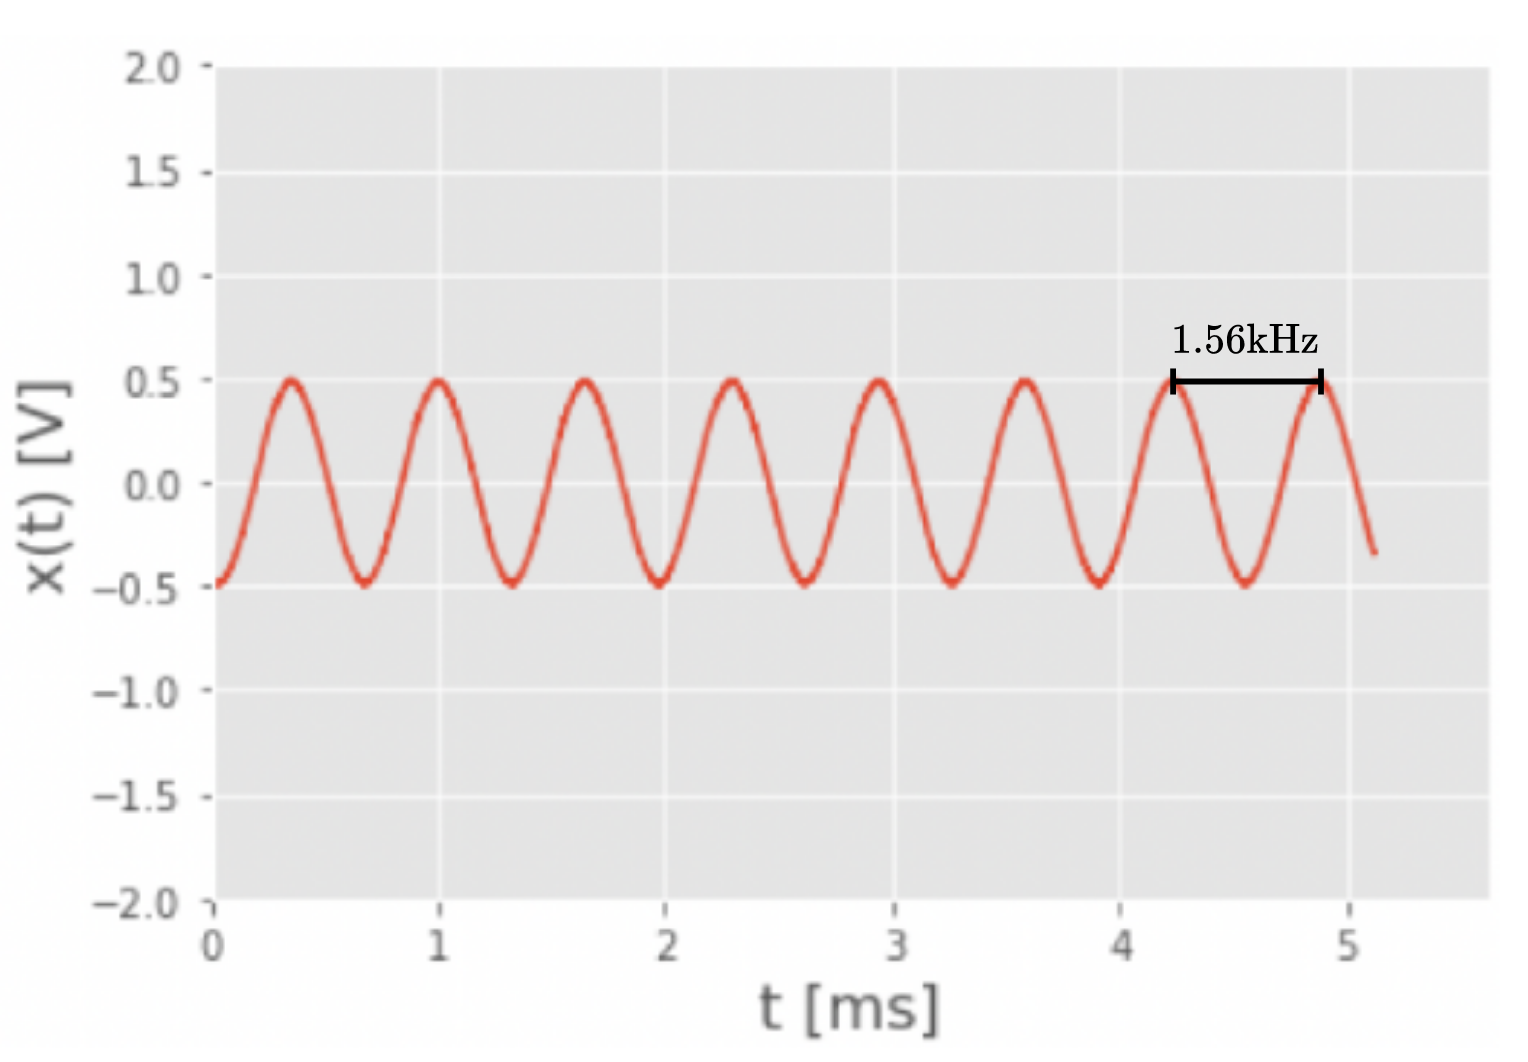
\includegraphics[width=0.75\textwidth]{img/Scope1_complete.png}
    \caption{Signalet $x(t)$ for $f_1$.}
    \label{fig: scope f_1}
\end{figure} \\
\begin{figure}[!htbp]
    \centering
    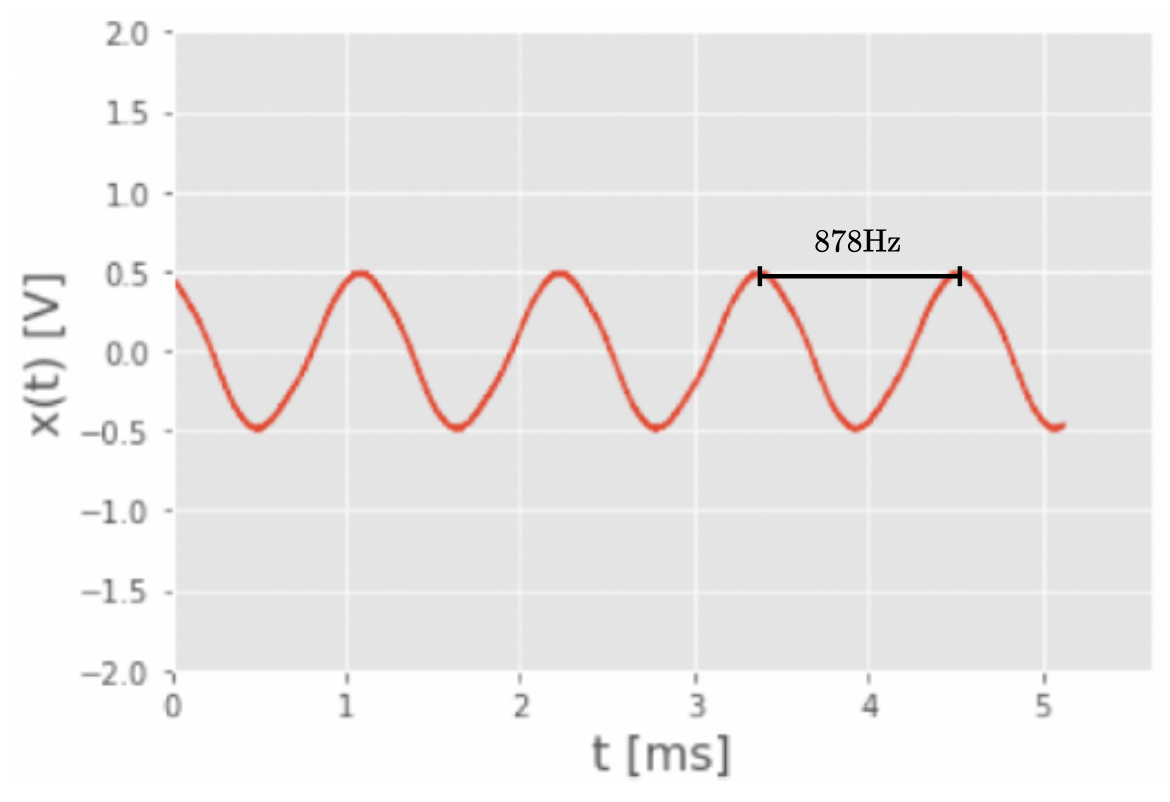
\includegraphics[width=0.75\textwidth]{img/Scope2_complete.png}
    \caption{Signalet $x(t)$ for $f_2$.}
    \label{fig: scope f_2}
\end{figure} \\
\newpage
\begin{figure}[!htbp]
    \centering
    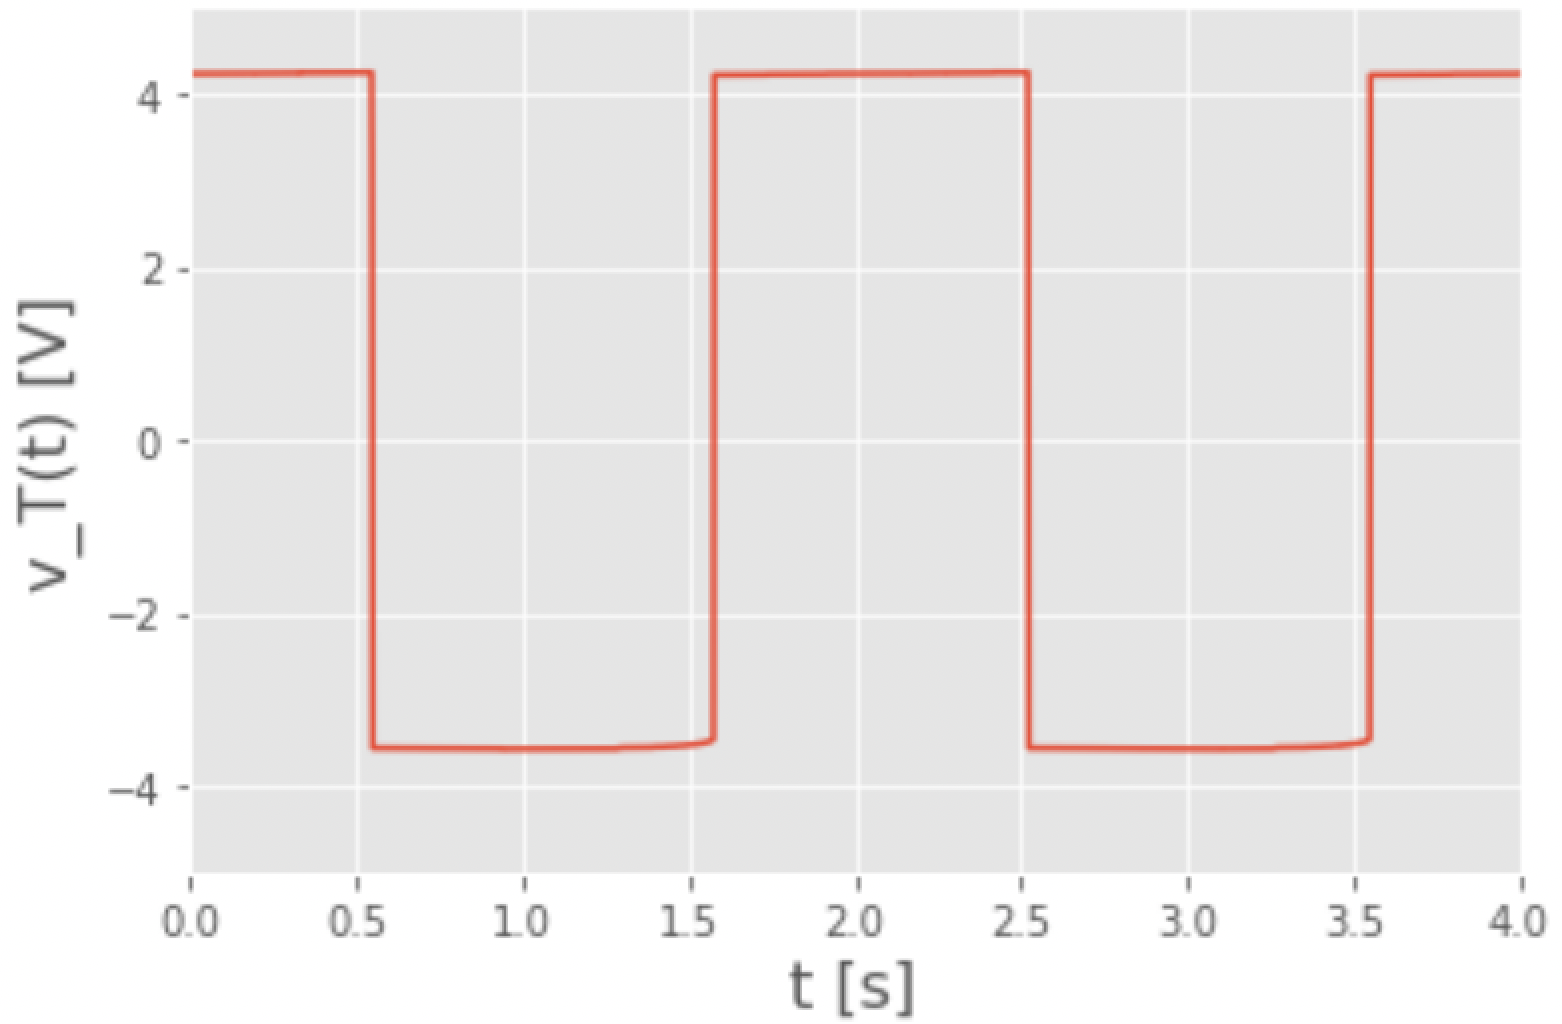
\includegraphics[width=0.75\textwidth]{img/Klokkesignal.png}
    \caption{Klokkesignalett til den tidsbestemte to-veis bryteren.}
    \label{fig: scope klokkesignal}
\end{figure} \\
Den realiserte modellen er vist i figur~\ref{fig: realisert modell}.
\begin{figure}[!htbp]
    \centering
    \includegraphics[width=0.75\textwidth]{img/Realisert krets.jpg}
    \caption{Realisert krets av figur~\ref{fig: avansert krets}.}
    \label{fig: realisert modell}
\end{figure} \\

\subsection{Overgang mellom $f_1$ og $f_2$}
Det kan være interessant å undersøke hva som skjer ved overgangen mellom frekvensene. Dette er vist for henholdsvis $f_1\rightarrow f_2$ og $f_2 \rightarrow f_1$ i figur~\ref{fig: f_1 til f_2 frekvensskifte} og figur~\ref{fig: f_2 til f_1 frekvensskifte}.
Her er det forstyrrelser ved overgangen, mest trolig fordi $f_1 \neq k \cdot f_2$, der $k$ er et heltall. Samtidig kan transistoren også forårsake støy i overgangen fordi overgangstiden mellom tilstandene ''på/av'' ikke kortslutter/åpner kretsen øyeblikkelig. \\
\begin{figure}[!htbp]
    \centering
    \includegraphics[width=0.75\textwidth]{img/Fra_hoy_til_lav_frekvensskifte.png}
    \caption{Området der $x(t)$ skifter fra $f_1$ til $f_2$.}
    \label{fig: f_1 til f_2 frekvensskifte}
\end{figure} \\
\begin{figure}[!htbp]
    \centering
    \includegraphics[width=0.75\textwidth]{img/Fra_lav_til_hoy_frekvensskifte.png}
    \caption{Området der $x(t)$ skifter fra $f_2$ til $f_1$.}
    \label{fig: f_2 til f_1 frekvensskifte}
\end{figure} \\
\newpage
\subsection{Effektspekteret}
For å få kontroll på 10-dB båndbredden, så analyserer vi effektspekteret. Dette resulterer i to relevante områder, slikt vist i figur~\ref{fig: effektspekteret}. \\
\begin{figure}[!htbp]
    \centering
    \includegraphics[width=0.75\textwidth]{img/Fullstendig_effektspekter.png}
    \caption{Effektspekteret $P_x(f)$ til $x(t)$.}
    \label{fig: effektspekteret}
\end{figure} \\
Skal vi analysere $B$, så er det lettere om vi zoomer inn på områdene rundt $f_1$ og $f_2$, slikt vist henholdsvis ved figur~\ref{fig: 10dBm for f_1} og figur~\ref{fig: 10dBm for f_2}. \\
\begin{figure}[!htbp]
    \centering
    \includegraphics[width=0.75\textwidth]{img/BP1_complete.png}
    \caption{10dBm-båndbredde for $f_1$.}
    \label{fig: 10dBm for f_1}
\end{figure} \\
\begin{figure}[!htbp]
    \centering
    \includegraphics[width=0.75\textwidth]{img/BP2_complete.png}
    \caption{10dBm-båndbredde for $f_2$.}
    \label{fig: 10dBm for f_2}
\end{figure} \\
Det er her små båndbredder på kun noen Hz i størrelse og det totale effektspekteret fra figur~\ref{fig: effektspekteret} viser forstyrrelser i høyere frekvenser, men ikke i en vesentlig grad. Siden det ikke er satt noe krav om kvaliteten (SNR) på $x(t)$, så vil de harmoniske frekvensene ikke ha noe betydning.
\\
\subsection{Effektforbruk}
Effektforbruk er gitt ved
\begin{equation}
    P = U \cdot I \: .
\end{equation} \\
Det er mulig å finne inngangsspenningen $U$ og strømmen $I$ hele kretsen trekker, ved et oscilloskop eller et voltemeter og amperemeter. Her brukes et programvare for å styre $V_+$ og $V_-$ til opampene, som er det eneste bidraget til effektforbruken kretsen har. Vi kan lese både spenningen og strømmen som påtrykkes opampene i oscilloskopet. Dette resulterer i at 
\begin{equation*}
    P = 5.065\textrm{V} \cdot 312\textrm{mA} = 1.58\textrm{W}.
\end{equation*}
Merk at dersom det legges til en opamp forsterker på systemet, så vil effektforbruket øke.
\subsection{Signalnivå når $R_L$ er tilkoblet}
Når det kobles på en lastmotstand $R_L$, så vil signalnivået for denne kretsen for respektivt $f_1$ og $f_2$ være gitt ved
\begin{equation}
    x_{dBV1} = 20\log_{10}\left(\frac{0.343\textrm{V}}{1\textrm{V}}\right) = -9.3\textrm{dBV},
\end{equation}
\begin{equation}
    x_{dBV2} = 20\log_{10}\left(\frac{0.343\textrm{V}}{1\textrm{V}}\right) = -9.3\textrm{dBV}.
\end{equation}
Disse signalene har samme verdi om det blir tilkoblet en $R_L$ eller ei, fordi det er en buffer før $x(t)$. Se neste avsnitt for forklaring. Dersom bufferen før $x(t)$ ikke er tilkoblet, så kan $R_L$ påvirke den tidsbestemte frekvensskifteren. Det siden $R_L$ er i parallell med $R_{H1}$ eller $R_{H2}$, avhengig av hvilken transistor som er aktiv. Dette kan forårsake et dempet $x(t)$ når lastmotstand er tilkoblet. 
\\\\
Bufferen resulterer i at det blir en lav utgangsimpedans $Z_o$, som er vanskelig å finne for dette systemet. Det fordi amplituden på den tidsbestemte frekvensskifteren ikke er helt stabil, men endres med noen mV over tid. En standard $Z_o$ for LF353N eksisterer i datablad. Se figur~\ref{fig: LF353N output impedance}. Grafen for $A_v = 1$ viser at $Z_o \in (0.03, 0.04)\Omega$. Merk at dersom det legges til en forsterker på signalet, så vil $Z_o$ øke. For å minke $Z_o$ igjen, så kan en buffer legges til etter forsterkeren. \\
\begin{figure}[!htbp]
    \centering
    \includegraphics[width=0.50\textwidth]{img/Output impedance.png}
    \caption{Utgangsimpedans (output impedance) for LF353-N \cite{LF353N Datasheet}.}
    \label{fig: LF353N output impedance}
\end{figure} \\
\newpage
\section{Konklusjon}
\label{sec: konklusjon}
Det utvikles en tidsbestemt frekvensskifter som er i stand til å skifte mellom to omtrentlige sinusfunksjoner med ulik frekvens. Frekvensene er ikke nærme de teoretisk utreknede verdiene, siden det er et ulineært system for oscillatoren. Området der frekvensene skifter har små forstyrrelser på rundt en periode, men holdes stabile etterpå. Systemet holder båndbreddene til frekvensene i underkant av $10$Hz ved bruk av båndpassfilter. Utgangsimpedansen er neglisjerbar på grunn av den analoge bufferen. Effektforbruket er på $1.58$W. Eventuelle forbedringer kan gjøres på klokkesignalet, der det kan brukes en ''crystal oscillator''. Det kan være hvis $f_1 = k\cdot f_2$, at overgangen mellom frekvensene kunne vært finere. Men det får vi ikke testet her. Dersom systemet setter krav på $x(t)$ som er bedre enn i \cite{U-oscillator}, så kan det være verdt å bruke en annerledes (mer komplisert) oscillator.


\newpage
%Bibliografi: Legg til flere elementer ved å legge til flere \bibitem:--------
\phantomsection
\addcontentsline{toc}{section}{Referanser}
\begin{thebibliography}{99}
\bibitem{U-oscillator} 
S. Danielsen (2021),  \\
''Designnotat 6: Ulineær Oscillator'', \\
Tilgjengelig ved: \\
Blackboard, TTT4265 Elektronisk systemdesign og -analyse II, NTNU.

\bibitem{Square wave generator} Elprocus (2021), \\ ''Square Wave Generator'', \\
Tilgjengelig ved: \\
\href{https://www.elprocus.com/what-is-a-square-wave-generator-circuit-diagram/}{https://www.elprocus.com/what-is-a-square-wave-generator-circuit-diagram/}

\bibitem{LF353N Datasheet} 
Texas Instruments (2013), \\
''LF353-N Wide Bandwidth Dual JFET Input Operational Amplifier'', \\
elektronisk datasheet, \\
Tilgjengelig ved: \\
\href{https://www.ti.com/lit/ds/symlink/lf353-n.pdf}{https://www.ti.com/lit/ds/symlink/lf353-n.pdf}.

\end{thebibliography}


\end{document}
